%%%%%%%%%%%%%%%%%%%%%%%%%%%%%%%%%%%%%%%%%
% Short Sectioned Assignment LaTeX Template Version 1.0 (5/5/12)
% This template has been downloaded from: http://www.LaTeXTemplates.com
% Original author:  Frits Wenneker (http://www.howtotex.com)
% License: CC BY-NC-SA 3.0 (http://creativecommons.org/licenses/by-nc-sa/3.0/)
%%%%%%%%%%%%%%%%%%%%%%%%%%%%%%%%%%%%%%%%%

%----------------------------------------------------------------------------------------
%	PACKAGES AND OTHER DOCUMENT CONFIGURATIONS
%----------------------------------------------------------------------------------------

\documentclass[paper=a4, fontsize=11pt]{scrartcl} % A4 paper and 11pt font size

% ---- Entrada y salida de texto -----

\usepackage[T1]{fontenc} % Use 8-bit encoding that has 256 glyphs
\usepackage[utf8]{inputenc}
%\usepackage{fourier} % Use the Adobe Utopia font for the document - comment this line to return to the LaTeX default

% ---- Idioma --------

\usepackage[spanish, es-tabla]{babel} % Selecciona el español para palabras introducidas automáticamente, p.ej. "septiembre" en la fecha y especifica que se use la palabra Tabla en vez de Cuadro

% ---- Otros paquetes ----

%https://en.wikibooks.org/wiki/LaTeX/Hyperlinks#.5Curl
\usepackage[colorlinks=true,linkcolor=blue,citecolor=red, urlcolor=blue]{hyperref} % para poder poner referencias, url...

%https://en.wikibooks.org/wiki/LaTeX/Colors
\usepackage{color, colortbl}
\usepackage[first=0,last=9]{lcg} %Color tabla
\newcommand{\ra}{\rand0.\arabic{rand}} %Color tabla

\usepackage{eurosym} %Símbolo del euro

\usepackage{amsmath,amsfonts,amsthm} % Math packages
%\usepackage{graphics,graphicx, floatrow} %para incluir imágenes y notas en las imágenes
\usepackage{graphics,graphicx, float, url} %para incluir imágenes y colocarlas

% Para hacer tablas comlejas
%\usepackage{multirow}
%\usepackage{threeparttable}

%\usepackage{sectsty} % Allows customizing section commands
%\allsectionsfont{\centering \normalfont\scshape} % Make all sections centered, the default font and small caps

\usepackage{fancyhdr} % Custom headers and footers
\pagestyle{fancyplain} % Makes all pages in the document conform to the custom headers and footers
\fancyhead{} % No page header - if you want one, create it in the same way as the footers below
\fancyfoot[L]{} % Empty left footer
\fancyfoot[C]{} % Empty center footer
\fancyfoot[R]{\thepage} % Page numbering for right footer
\renewcommand{\headrulewidth}{0pt} % Remove header underlines
\renewcommand{\footrulewidth}{0pt} % Remove footer underlines
\setlength{\headheight}{13.6pt} % Customize the height of the header

\numberwithin{equation}{section} % Number equations within sections (i.e. 1.1, 1.2, 2.1, 2.2 instead of 1, 2, 3, 4)
\numberwithin{figure}{section} % Number figures within sections (i.e. 1.1, 1.2, 2.1, 2.2 instead of 1, 2, 3, 4)
\numberwithin{table}{section} % Number tables within sections (i.e. 1.1, 1.2, 2.1, 2.2 instead of 1, 2, 3, 4)

\setlength\parindent{0pt} % Removes all indentation from paragraphs - comment this line for an assignment with lots of text

\newcommand{\horrule}[1]{\rule{\linewidth}{#1}} % Create horizontal rule command with 1 argument of height

\usepackage{enumerate}
\usepackage{listings}
\usepackage{amsmath}%
\usepackage{amsfonts}%
\usepackage{amssymb}%
\usepackage{MnSymbol}%
\usepackage{wasysym}%
\usepackage{graphicx}
\usepackage{grffile}
\usepackage[spanish]{babel}
\usepackage{babel}
\usepackage{tikz}
\usetikzlibrary{babel}
\usepackage{color}
\usepackage{hyperref}

\definecolor{dkgreen}{rgb}{0,0.6,0}
\definecolor{gray}{rgb}{0.5,0.5,0.5}
\definecolor{mauve}{rgb}{0.58,0,0.82}

\lstset{frame=tb,
	language=Java,
	aboveskip=3mm,
	belowskip=3mm,
	showstringspaces=false,
	columns=flexible,
	basicstyle={\small\ttfamily},
	numbers=none,
	numberstyle=\tiny\color{gray},
	keywordstyle=\color{blue},
	commentstyle=\color{dkgreen},
	stringstyle=\color{mauve},
	breaklines=true,
	breakatwhitespace=true,
	tabsize=3
}

%----------------------------------------------------------------------------------------
%	TÍTULO Y DATOS DEL ALUMNO
%----------------------------------------------------------------------------------------

\title{
\normalfont \normalsize
\textsc{ Programación de Dispositivos Móviles (2017-2018)\\
			Grado en Ingeniería Informática\\ 
			Universidad de Granada}
			\\ [25pt] % Your university, school and/or department name(s)
\horrule{0.5pt} \\[0.4cm] % Thin top horizontal rule
\huge Tutorial 1\\ % The assignment title
\horrule{2pt} \\[0.5cm] % Thick bottom horizontal rule
}

\author{ Juan Alberto Martínez López \\ Alberto Armijo Ruiz \\}

\date{2 de abril de 2018} % Incluye la fecha actual



%----------------------------------------------------------------------------------------
% DOCUMENTO
%----------------------------------------------------------------------------------------

\begin{document}

\maketitle % Muestra el Título


\includegraphics[width=1\linewidth]{ugr}

\newpage %inserta un salto de página

\tableofcontents % para generar el índice de contenidos

%\listoffigures

%\listoftables

\newpage

%----------------------------------------------------------------------------------------
%	Introducción
%----------------------------------------------------------------------------------------

\section*{Introducción}

Para esta práctica 


\section{Evaluación de tiempos}


\begin{table}[htbp]
	\begin{center}
		\begin{tabular}{|l|l|l|l|}
			A & B & P & Tiempos (s) \\ \hline
			6 & 50628 & 57347 & 0.001187 \\ \hline 
			8 & 449605 & 468577 & 0.004052 \\ \hline
			207 & 4374842 & 5555567 & 0.018117 \\ \hline
			4007 & 8515459 & 87654337 & 0.080128\\ \hline
			40756 & 118205788 & 987654323 & 0.289543\\ \hline
			20544 & 253647140 & 3141592661 & 0.735911\\ \hline
			112354 & 9048018943 & 11111111113 & 1.506318\\ \hline
			1245628 & 49579028347 & 121212121223 & 5.264323\\ \hline
			87569 & 1342094524016 & 2718281828489 & 29.752512\\ \hline
			568236 & 14717101287551 & 16180339892149 & 76.744032\\ \hline
			4555786 & 778596955901441 & 800000000000017 & 612.546521\\ \hline
		\end{tabular}
		\caption{Tabla análisis de logaritmo.}
		\label{tabla:compleja}
	\end{center}
\end{table}

\begin{table}[htbp]
	\begin{center}
		\begin{tabular}{|l|l|}
			Longitud clave & Tiempo ejecución (seg) \\ \hline
			5 & 0.001187 \\ \hline 
			6 & 0.004052 \\ \hline
			7 & 0.018117 \\ \hline
			8 & 0.080128\\ \hline
			9 & 0.289543\\ \hline
			10 & 0.73591\\ \hline
			11 & 1.506318\\ \hline
			12 & 5.264323\\ \hline
			13 & 29.752512\\ \hline
			14 & 76.744032 \\ \hline
			15 & 612.546521\\ \hline
		\end{tabular}
		\caption{Tabla tiempos}
		\label{tabla:resumen}
	\end{center}
\end{table}


\begin{figure}[H]
	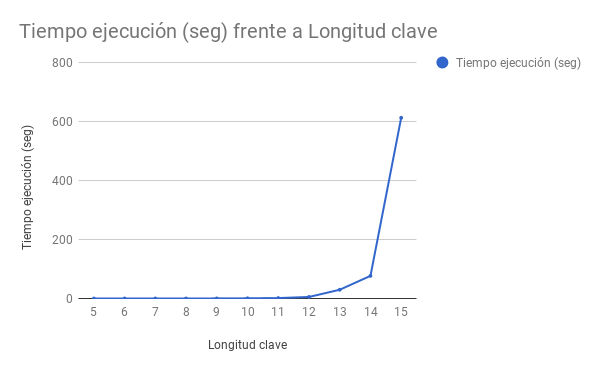
\includegraphics[width=1\linewidth]{chart}
	\caption{Tiempos vs Longitud clave}
\end{figure}
%\includegraphics[width=1\linewidth]{Capturas VRTK/prueba 43.1}\\

%\includegraphics[width=1\linewidth]{Capturas VRTK/prueba 43.2}\\

%\includegraphics[width=1\linewidth]{Capturas VRTK/prueba 43.3}


%----------------------------------------------------------------------------------------
%	REFERENCIAS
%----------------------------------------------------------------------------------------

%\section{Incluyendo las referencias}

%A lo largo del texto, tendrá que incluir referencias, para ello puede usar las
%notas a pie de página con \textbackslash footnote \footnote{Este es un ejemplo}
%o añadiendo citas con \textbackslash cite \cite{mrx05,prueba2}.
%\LaTeX puede gestionar las referencias mediante BibTex, que genera entradas bbl
%a partir de un archivo .bib. También puede incluirlas directamente en el documento
%fuente como entradas dentro de una sección (thebibliography) dentro del mismo
%documento (son las generadas en el archivo .bbl por BibTex). No obstante,
%se recomienda el uso del archivo .bib como buena práctica a seguir cuando se
%trabaje con \LaTeX.

%Para incluir las referencias usaremos la etiqueta \textbackslash bibliography
%especificando su estilo: \textbackslash bibliographystyle que, en nuestro caso,
%es plain.

%------------------------------------------------
%\newpage

%\bibliographystyle{plain} % hay varias formas de citar

%\begin{thebibliography}{99} %Principio Bibliografía (99 max elementos)

	%\bibitem{virtual} Virtualización. (24 de septiembre de 2015):
	%\url{http://www.vmware.com/latam/virtualization/how-it-works}.

%	\bibitem{proyectivo} \url{http://www.rac.es/ficheros/doc/00894.pdf} 
%	\bibitem{consP} \url{https://eva.fing.edu.uy/pluginfile.php/63526/mod_resource/content/2/Teorico/clase04_TransformacionesGeo.pdf}
%	\bibitem{homomorfismo} \url{https://en.wikipedia.org/wiki/Homography#Homographies_of_a_projective_line}
%	\bibitem{hart} Multiple View Geometry in Computer Vision (Second Edition) \textit{Richard Hartley, Andrew Zisserman}
%	\bibitem{szel} Computer vision: Algorithms and applications \textit{Richard Szeliski}	

%\end{thebibliography}


%\bibliography{citas} %archivo citas.bib que contiene las entradas




\end{document}